\subsection{Metrický prostor}
Metrický prostor je \textbf{matematická struktura}, pomocí které lze formálním způsobem definovat pojem \textbf{vzdálenosti}. Na metrických prostorech se poté definují další topologické vlastnosti jako např. \textbf{otevřenost} a \textbf{uzavřenost} množin, jejichž zobecnění pak vede na ještě abstraktnější matematický pojem \textbf{topologického prostoru}.

\subsubsection{Formální definice}
Metrický prostor je dvojice $(M, \rho)$, kde $M$ je libovolná neprázdná množina a $\rho$ je \textbf{metrika}, což je zobrazení:
\begin{equation*}
\rho: M \times M \rightarrow \mathbb{R},
\end{equation*}
které splňuje následující axiomy:
\begin{enumerate}
\item \textbf{Nezápornost}: $\forall x, y \, \rho(x, y) \geq 0$.
\item \textbf{Totožnost}: $\forall x, y \, \rho (x, y)  = 0 \Leftrightarrow x = y$.
\item \textbf{Symetrie}: $\forall x, y \in M: \, \rho(x, y) = \rho(y,x)$.
\item \textbf{Trojúhelníková nerovnost}: $\forall x, y, z \in M: \, \rho(x, y) + \rho(y,z) \geq \rho(x, y)$.
\end{enumerate}

\subsubsection{Metriky v $\mathbb{R}^n$}
U metrik v $\mathbb{R}^n$ platí:
\begin{itemize}
\item Každý normovaný vektorový prostor je metrickým prostorem.
\item Množina reálných čísel spolu s metrikou $\rho(x, y) = |x - y|$, kde $x, y$ jsou libovolné body množiny $\mathbb{R}$ tvoří \textbf{úplný metrický prostor}.
\end{itemize}
Mezi nejpoužívanější \textbf{metriky} na Euklidovském prostoru $\mathbb{R}^n$ patří:
\begin{enumerate}
\item \textbf{Manhattanská} -- $\rho_1(x, y) = \sum_{i = 0}^n |x_i - y_i|$.
\item \textbf{Euklidovská} -- $\rho_2(x, y) = \sqrt{\sum_{i = 0}^n |x_i - y_i|^2}$.
\item \textbf{Minkowského} -- $\rho_3(x, y) = (\sum_{i = 0}^n |x_i - y_i|^P)^{1/P}$, kde $P \geq 1; \, P \in \mathbb{R}$.
\item \textbf{Čebyševova (Maximova)} -- $\rho_{\max}(x, y) = \max_{\forall i} |x_i - y_i|$, speciální případ Minkowského metriky pro $P = \infty$.
\end{enumerate}

\subsubsection{Podobnosti a nepodobnosti}
\begin{itemize}
\item \textbf{Cosinova podobnost} -- míra podobnosti dvou vektorů, která se získá výpočtem kosinu úhlu těchto vektorů:
\begin{equation*}
S_c(x, y) = \frac{x \cdot y}{||x|| \, ||y||} = \frac{\sum_{i = 0}^{n} x_i - y_i}{\sqrt{\sum_{i = 0}^{n} x_i^2} \sqrt{\sum_{i = 0}^{n} y_i^2}}
\end{equation*}
\item \textbf{Jaccardova podobnost} -- $S_j(X, Y) = \frac{|X \cap Y|}{X \cup Y}$ používá se pro porovnání podobnosti dvou množin.
\item \textbf{Jaccardova nepodobnost} (svým způsobem vzdálenost) -- $d = 1 - S$, $d = \frac{1}{S} - 1$ pro $S \neq 0$.
\end{itemize}

\subsubsection{Vzdálenost mezi slovy}
K určení vzdálenosti mezi textovými řetězci definujeme tyto \textbf{vzdálenosti}:
\begin{enumerate}
\item \textbf{Hammingova} -- počet rozdílných písmen na stejných pozicích: $d_h(\textrm{Karolin, Kathrin}) = 3$, lze použít pouze pro \textbf{stejně dlouhá slova!}.
\item \textbf{LCS (Longest common subsequence)} -- počet operací \textbf{vkládání} a \textbf{mazání} nutných k převodu jednoho slova na druhé: $d_{\textrm{LCS}	}(\textrm{kitten, sitting}) \Rightarrow \textrm{itten [-K]} \rightarrow \textrm{sitten [+S]} \rightarrow \textrm{sittn [-E]} \rightarrow \textrm{sittin [+I]} \rightarrow \textrm{sitting [+G]} =$ \textbf{5 operací}.
\item \textbf{Levenshteinova} -- počet operací \textbf{vkládání}, \textbf{mazání}, \textbf{substituce}  nutných k převodu jednoho slova na druhé: $d_l(\textrm{kittne, sitting}) \Rightarrow \textrm{sitten [K }\sim \textrm{ S]} \rightarrow \textrm{sittin [E }\sim \textrm{ I]} \rightarrow \textrm{sitting [+G]} =$ \textbf{3 operace}.
\end{enumerate}
\textbf{Editační vzdálenost} patří zde LSC a Levenstheinova vzdálenost (při určení se používají úpravy).

\subsubsection{Normalizace}
Snažíme se dostat všechny hodnoty atributů ve sloupci do intervalu $\langle 0, 1\rangle$, proto dělíme celý sloupce jeho maximem (dělíme v rámci daného sloupce, pro každý sloupec zvlášť vlastním maximem).

\subsubsection*{Příklad}
$d'_1$ a $d'_2$ reprezentují \textbf{normovaný tvar} vzdáleností $d_1$ a $d_2$:
\begin{table}[H]
\centering
\begin{tabular}{l|lllllll}
	& $t_1$ &  $t_2$ & $t_3$ & $t_4$ &$t_5$  & $t_6$ &$t_7$  \\\hhline
	$d_1$&  1& 0 &0  &  1&3  &  0&1  \\
	$d_2$&  1&  0&  0&  2&  2& 0 & 0 \\
	$d'_1$&  1&  0&  0&  $\frac{1}{2}$& 1 &  0& 1 \\
	$d'_2$&  1&  0&  0&  1& $\frac{2}{3}$ &  0& 0
\end{tabular}
\end{table}
\begin{table}[H]
\centering
\begin{tabular}{l|l|l|l|l|l|l}
	& $i = 1$ &  $i = 2$ & $i = 3$ & $i = \infty$ &Cosinova  & Jaccard  \\\hhline
	$\rho_i(d_1, d_2)$&   3 &$\sqrt{3}$  &  $ \sqrt{3}^3 $&1 &  $\frac{1}{6 \sqrt(3)}$& $\frac{3}{4}?$ \\
	$\rho_i(d'_1, d'_2)$&   $\frac{11}{6}$&  $\frac{7}{6}$& $\frac{3 \sqrt{251}}{6}$&  1& $\frac{5 \sqrt(154)}{3 \sqrt(2)}$ & $\frac{3}{4}?$
\end{tabular}
\end{table}

\subsection{Topologický prostor}
Jedná se o \textbf{rozšíření (zobecnění) metrického prostoru}. Cílem topologie je studium \textbf{vlastností prostorů}. Na rozdíl od teorie metrických prostorů se v topologii \textbf{nezajímáme o vzdálenosti mezi body} prostoru a prostory považujeme za stejné, pokud \textbf{se na sebe dají vzájemně přeměnit} nějakou spojitou deformací. Takže např. nerozlišujeme mezi koulí a krychlí, ostatně koule se změní v krychli již při přechodu mezi dvěma ekvivalentními metrikami v $\mathbb{R}^3$.

Základním pojmem, který se v topologii studuje je \textbf{spojitost zobrazení}. Proto není úplně potřeba vědět přesně, jak jsou od sebe které body daleko. Vystačíme si s informacemi, že jisté body se nekonečně blíží k nějakému bodu prostoru.

\subsubsection{Formální definice}
Topologickým prostorem nazveme množinu $X$ společně s kolekcí $\tau$ podmnožin $X$, tedy \textbf{dvojici} $(X, \tau)$, splňující následující axiomy:
\begin{enumerate}
\item $\emptyset, X \in \tau$,
\item $\forall A, B \in \tau \Rightarrow  A \cup B \in \tau $, tedy \textbf{sjednocení} libovolného počtu (tj. konečného, spočetného i nespočetného) množin z $\tau$ leží v $\tau$,
\item $\forall A, B \in \tau \Rightarrow A \cap B \in \tau $, tedy \textbf{průnik} konečného počtu množin z $\tau$ leží v $\tau$.
\end{enumerate}

\subsubsection{Uzavřená, otevřená množina}
\begin{minipage}[t]{0.49\textwidth}
$A \in \tau$ \ldots A je \textbf{otevřená} pokud:
\begin{itemize}
\item $\emptyset, X \in \tau$,
\item $\forall A, B \in \tau \Rightarrow  A \cap B \in \tau $,
\item $\forall A_i \in \tau \Rightarrow \cup A_i \in \tau $.
\end{itemize}
$\cup A_i \Leftrightarrow A_1 \cup A_2 \cup ... \cup A_n $
\end{minipage}
\begin{minipage}[t]{0.49\textwidth}
$A \in \tau$ \ldots A je \textbf{uzavřená} pokud:
\begin{itemize}
\item $\emptyset, X \in \tau$,
\item $\forall A, B \in \tau \Rightarrow  A \cup B \in \tau $,
\item $\forall A_i \in \tau \Rightarrow \cap A_i \in \tau $.
\end{itemize}
$\cap A_i \Leftrightarrow A_1 \cap A_2 \cap ... \cap A_n $
\end{minipage}

\subsubsection{Souvislost nesouvislost}
Pokud sjednocením dvou neprázdných množin z $\tau$ získáme všechny prvky topologie (celé $ X $), tak je topologie \textbf{nesouvislá}. Příklad:

\begin{center}
\begin{minipage}[t]{0.50\textwidth}
	$X = \{a, b, c\}$\\
	$\tau = \{\emptyset, X, \{a, b\}, \{c\}\}$\\
	$\{a, b\} \cup \{c\}  = \{a, b, c\} \Rightarrow \, \tau$ je \textbf{nesouvislá}
\end{minipage}
\begin{minipage}[t]{0.40\textwidth}
	\textbf{Poznámka:} sjednocované množiny musí být \textbf{disjunktní}, tedy nesmí mít společné prvky, např.: $\{a, b\}$ a $\{a, c\}$ již disjunktní nejsou, ale nenaruší souvislost.
\end{minipage}
\end{center}
\smallskip
Topologický prostor $ \tau $, je \textbf{souvislý} právě tehdy, když jedině podmnožiny v $\tau$, které jsou současně otevřené i uzavřené jsou $X$ a $\emptyset$. V opačném případě je $\tau$ \textbf{nesouvislý}.

\subsubsection{Uzávěrový systém}
Uzávěrový systém $C$ nad množinou $X$ obsahuje $X$ a $\forall A, B \in C$ platí, že $A \cap B \in C$.
\begin{equation*}
\begin{aligned}
R_i \subseteq A \times A \quad R_i^* = \textrm{[tranzitivně-reflexivní uzávěr]}\\
\textrm{pro } R_i^* \textrm{ platí } \quad R_1^* \neq R_2^*; \quad R_1^* \cap R_2^* \in G;\quad R_1^* \cup R_2^* \notin G
\end{aligned}
\end{equation*}

\subsubsection{Uzávěrový operátor $cl(A)$}
Uzávěr (\textit{closure}) $A \cup C \rightarrow cl(A)$ je \textbf{nejmenší uzavřená množina obsahující daný prvek}. Analogie u konceptů $cl(B) = B^{\downarrow\uparrow}$ a $cl(A) = A^{\uparrow\downarrow}$. Vlastnosti uzávěrového operátoru:
\begin{enumerate}
\item \textbf{Idempotence} -- $cl(cl(A)) = cl(A)$.
\item \textbf{Extensionalita} -- $A \subseteq cl(A)$.
\item \textbf{Monotónost} -- $A \subseteq B \Rightarrow cl(A) \subseteq cl(B)$.
\end{enumerate}

Platí-li navíc $cl(\emptyset) = \emptyset$ a $cl(A \cup B) = cl(A) \cup cl(B)$, pak je uzávěr $A = cl(A)$. Jinými slovy se jedná o nejmenší komplement (doplněk) množin TP obsahující daný prvek.
\\
\begin{figure}[H]
	\centering
	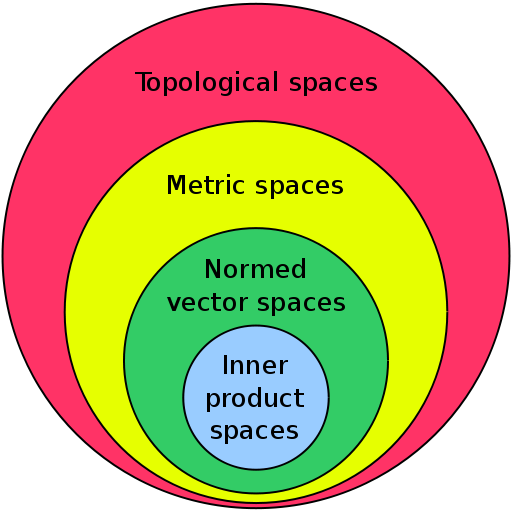
\includegraphics[width=0.4\textwidth]{assets/9_tpl_space}
\end{figure}


